% @Author: AnthonyKenny98
% @Date:   2020-03-01 19:39:42
% @Last Modified by:   AnthonyKenny98
% @Last Modified time: 2020-04-09 18:42:38

% Intro
Computer Architecture encompasses the design of the Instruction Set Architecture and Microarchitecture of a computer. The Instruction Set defines an abstract model of a computer, i.e. how it behaves. Microarchitecture is the implementation of this abstract model, i.e. desiging a CPU to execute the behavious specified in the instruction set.

% @Author: AnthonyKenny98
% @Date:   2020-04-09 10:47:05
% @Last Modified by:   AnthonyKenny98
% @Last Modified time: 2020-04-09 11:21:26
\begin{figure}[H]
\begin{centering}
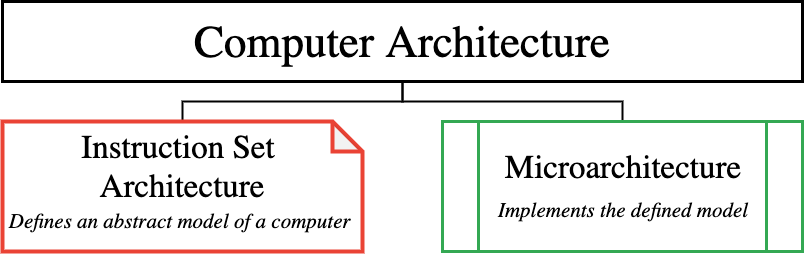
\includegraphics[width=0.7\linewidth]{chapters/chapter4/img/architecture.png}
\mycaption{Overview of the Field of Computer Architecture}{}
\end{centering}
\end{figure}

\subsection{Instruction Set Architecture}
    An \glsfirst{ISA} is an abstract model of a computer. On a broad level, it defines the data types, memory model, and registers of a computer, along with the instructions that it can execute. \\
    In more human terms, it can be thought as a ``contract'' between hardware and software developers. It is the promise made that the hardware will be able to execute all instructions defined in the \gls{ISA}, and the limitation that software must be compiled into that set of instructions.

    % @Author: AnthonyKenny98
% @Date:   2020-04-09 10:47:05
% @Last Modified by:   AnthonyKenny98
% @Last Modified time: 2020-04-11 01:21:24
\begin{figure}[H]
\begin{centering}
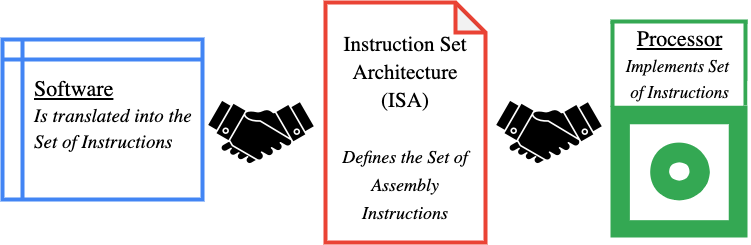
\includegraphics[width=\linewidth]{chapters/chapter4/img/contract.png}
\mycaption{The ISA is a Contract Between Software and Hardware Developers}{}
\end{centering}
\end{figure}

    The two most important things an \gls{ISA} defines are a computers \textbf{registers} and \textbf{instructions}. Instructions are the operations the computer can execute. Consider the \texttt{add} instruction: \texttt{add rd, rs1, rs2}

    This instruction computes \texttt{rs1} $+$ \texttt{rs2} and stores the result in \texttt{rd}.  \texttt{rd}, \texttt{rs1}, and \texttt{rs2} are all \textbf{registers}.
    
\subsection{Reduced Instruction Set Computer (RISC)}
    There are two broad classifications of \glspl{ISA}: \glsfirst{CISC} and \glsfirst{RISC}. Table \ref{table:CISCvRISC} outlines the key differences between the two.

    % @Author: AnthonyKenny98
% @Date:   2020-04-09 11:26:10
% @Last Modified by:   AnthonyKenny98
% @Last Modified time: 2020-04-09 18:23:43
\begin{table}[H]
\begin{centering}
\begin{tabular}{|m{0.45\linewidth}|m{0.45\linewidth}|}
\hline
\textbf{CISC} & \textbf{RISC} \\
\hline
Emphasis on Hardware Implementation 
    & Emphasis on Software \\
\hline
Multi-cycle, complex instructions. Different Instructions take different amounts of time to execute.
    & Single-cycle, simple instructions. All base instructions take the same amount of time to execute. \\
\hline
Operations can be performed directly on values stored in memory. 
    & Memory must be loaded into registers, operated on, and then stored back into memory. \\
\hline
Higher number of cycles per second 
    & Lower number of cycles per second \\
\hline
Smaller Assembly code sizes
    & Larger code sizes \\
\hline
\end{tabular}
\mycaption{Comparison of CISC and RISC ISAs.}{The operating philosophy of the two can really be broken down as follows: CISC has more complex instructions, higher cycles per second, and more cycles per instruction. RISC has fewer, more simple instructions, fewer cycles per second, and generally only one execution cycle per instruction.}
\end{centering}
\end{table}

\subsection{RISC Microarchitecture}
    
    Figure \ref{fig:RISC-Datapath} shows the most simple layout of a 5-stage RISC Datapath. In the \textbf{Instruction Fetch} stage, the processor gets the next instruction from memory for it to be decoded in the \textbf{Instruction Decode} stage. Here, the instruction is split into its constituent parts and has certain minor operations performed that are neccesary for the next stage. The \textbf{Execution} stage is where most computation occurs. This is where the \glsfirst{ALU} resides, and the result of this computation goes to the \textbf{Memory} stage. This is where values are stored into or loaded from the processor's memory, these values, or the values from the Execution stage, are saved to one of the processor's registers in the \textbf{Writeback} stage. 
    % @Author: AnthonyKenny98
% @Date:   2020-03-01 20:09:46
% @Last Modified by:   AnthonyKenny98
% @Last Modified time: 2020-04-03 13:32:58
\begin{figure}[H]
    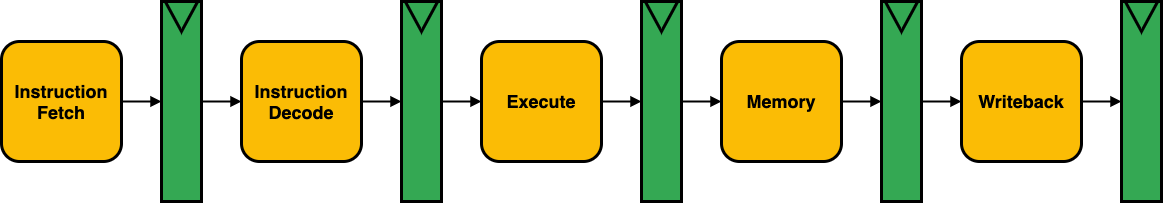
\includegraphics[draft=false,width=\linewidth]{chapters/chapter4/img/RISC-Datapath.png}
    \caption{5-Stage \gls{RISC} Datapath}
    \label{fig:RISC-Datapath}
\end{figure}
